%%%%%%%%%%%%%%%%%%%%%%%%%%%%%%%%%%%%%%%%%%%%%%%%%%%%%%%%%%%%%%%%%%%%%%%%%%%%%%%%
\section{Results}


\begin{figure}[t!]
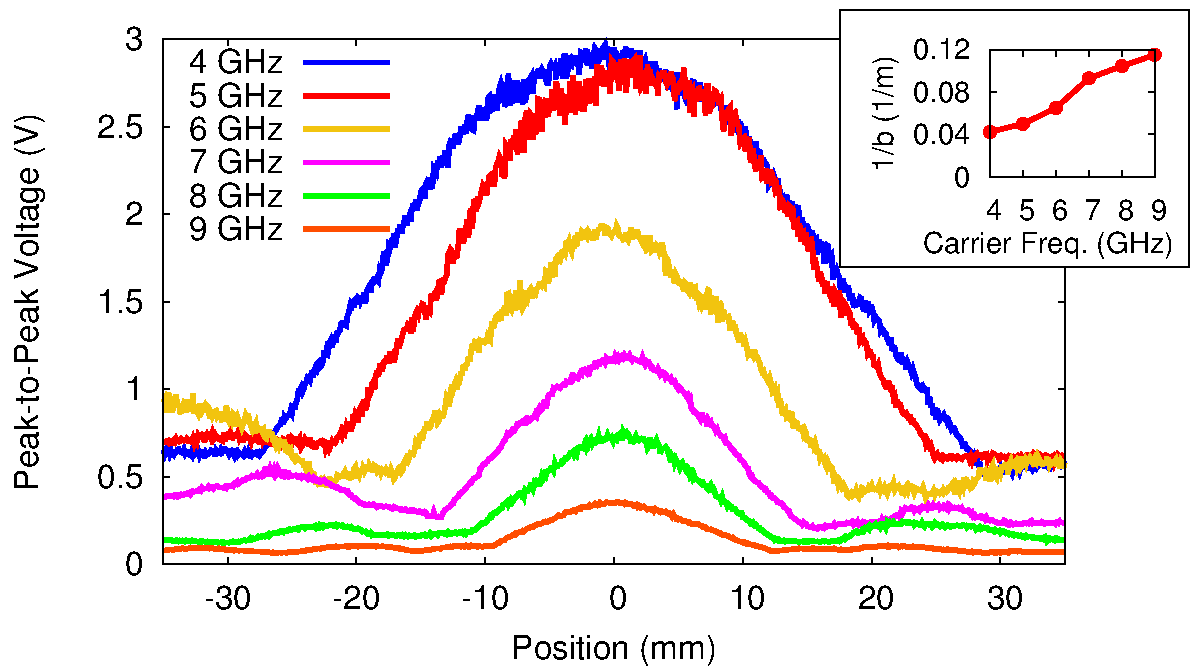
\includegraphics[width=\columnwidth]{figs/freq_profile.pdf}
\caption{Spatial profile of peak-to-peak voltage amplitudes of reconstructions
at carrier frequencies ranging from \numrange{4}{9}~GHz in 1~GHz
steps. The inset shows the inverse of the fit $b$ value versus carrier
frequency, showing the expected linear relationship. Differences in amplitude
are due to differences in $S_{1,2}$ parameters between frequencies for our particular antennas.}
\label{fig:freq_profile}
\end{figure}


%%%%%%%%%%%%%%%%%%%%%%%%%%%%%%%%%%%%%%%%%%%%%%%%%%%%%%%%%%%%%%%%%%%%%%%%%%%%%%%%
\subsection{Spatial Profiling}
\label{sec:spatial}

The first experiment conducted measures the spatial profile of a reconstruction
with the goal of characterizing reconstruction size as a function of carrier
signal wavelength.
%
Initially, a reconstruction is focused on the receiving antenna in the middle of its
movement range.
%
Without changing the time reversed sona being broadcast, the receiving antenna
is systematically translated through its entire range of movement.
%
Samples are taken every 0.2~mm across the entire 70~mm range and the
maximum peak-to-peak voltage of the corresponding reconstruction is recorded at
each step.
%
We repeated this experiment for carrier frequencies in the range
\numrange{4}{9}~GHz and display these results in Fig.~\ref{fig:freq_profile}.



The reconstruction peak-to-peak voltage profile is expected to take the form of
a $\left|sinc(x)\right|$ function about the antenna~\cite{lerosey-focusing}.
%
Thus, the following equation is proposed to predict $V(x)$, the maximum
peak-to-peak voltage from a given reconstruction, as a function of $x$, the
distance between the reconstruction focal point and the receiver:
%
\begin{equation}\label{eq:vx}
V(x)=a\cdot \left|sinc\left(\frac{x+c}{b}\right)\right|+d\,,
\end{equation}
%
\noindent where $a$ is the maximum peak-to-peak reconstruction amplitude, $b$ is
the wavelength of the signal divided by $2\pi$, $c$ is the location of the
antenna along the $x$-axis, and $d$ is the noise-level offset voltage.



Since $b$ is proportional to the wavelength (and inversely proportional to
frequency), as the carrier frequency is increased, $\frac{1}{b}$ also increases,
causing the main lobe of the $\left|sinc(x)\right|$ function in
Fig.~\ref{fig:freq_profile} to get smaller.
%
This relationship is shown explicitly in the inset of
Fig.~\ref{fig:freq_profile}.



Fig.~\ref{fig:error_fit} shows Equation~\ref{eq:vx} fit to the 5~GHz curve from
Fig.~\ref{fig:freq_profile}, including error bars.
%
This fit has a reduced $\chi^2$ of $234$ due in part to the rather
large background noise level.
%
The error bars are primarily systematic, introduced by the oscilloscope's internal
voltage multiplier used in scaling.
%%%%%%%%%%%%%%%%%%%%%%%%%%%%%%%%%%%%%%%%%%%%%%%%%%%%%%%%%%%%%%%%%%%%%%%%%%%%%%%%

%%%%%%%%%%%%%%%%%%%%%%%%%%%%%%%%%%%%%%%%%%%%%%%%%%%%%%%%%%%%%%%%%%%%%%%%%%%%%%%%
\subsection{Moving Reconstructions}
\label{sec:moving}


\begin{figure}[t!]
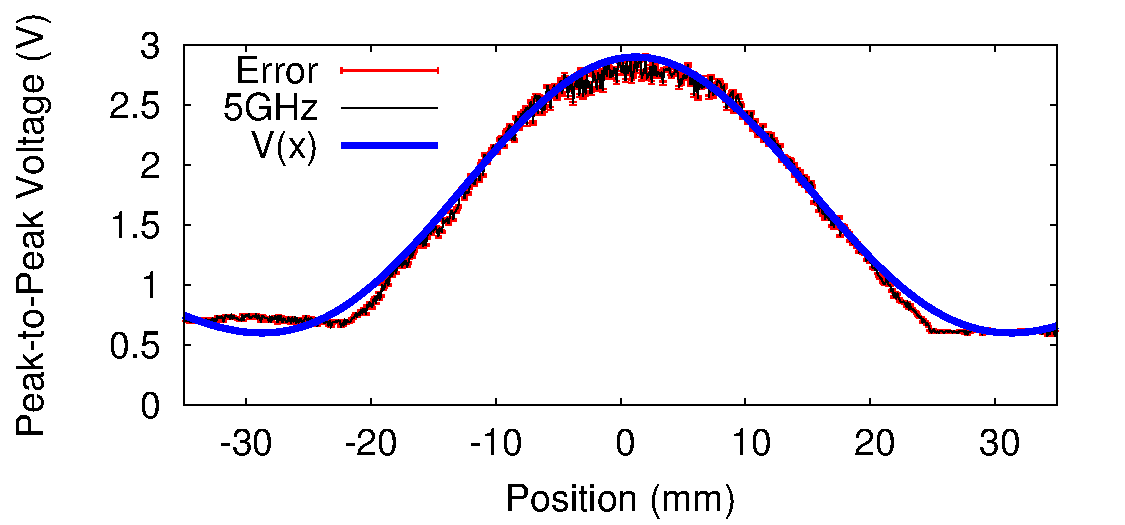
\includegraphics[width=\columnwidth]{figs/fit.pdf}
\caption{Measured peak-to-peak voltage amplitude of reconstructions received in the
vicinity of a time reversed wave collapse location with a 5 GHz carrier
frequency, and fit to Eq.~\ref{eq:vx}}
\label{fig:error_fit}
\end{figure}


The time reversal process assumes that the environment remains fixed between the
time-forward and time reversed steps.
%
It also assumes that the source and target remain fixed between these two steps.
%
We performed time reversal on a moving target to better understand how a
translating target affects reconstruction strength.



For this experiment, the receiving antenna moved at a constant speed of
0.5~$\frac{mm}{s}$ across the entire 70~mm range provided by the MikroMove.
%
To counteract the degradation of reconstruction strength as the antenna moved,
we periodically repeated the interrogation step, effectively re-centering the
reconstruction on the antenna.
%
Since the test equipment does not allow broadcast of one sona while collecting
another, it was not possible to transmit power during the collection time,
leading to a finite ``dead time'', denoted $t_d$ in Fig.~\ref{fig:moving_recon}.
%
During the broadcast period, the time reversed sona was continually broadcast
into the cavity (once every 15~$\mu s$) and the peak-to-peak voltage across the
receiver was measured once every 2.05~seconds, meaning that the reconstructions
are highly under-sampled in this plot.
%
After 15~samples were collected, we initiated the collection of a new sona, processed and rebroadcast it, and
began again. We refer to this full process of collecting a new sona and
then broadcasting it for a given period time as a full ``cycle'' of length
$t_c$.
%
The results in Fig.~\ref{fig:moving_recon} were obtained using a carrier
frequency of 5~GHz, $t_d$ of 7~seconds, and $t_c$ of 39.8~seconds.



Based on the results from Section~\ref{sec:spatial}, the peak-to-peak
reconstruction voltage measured by the receiver is expected to decay according
to the $\left|sinc(x)\right|$ function as the receiver moves away from the
reconstruction focal point.
%
This $\left|sinc(x)\right|$ function will be centered on the position where the sona
was last collected, making the reconstruction focus continually lag behind the
antenna.
%
Consequently, the maximum reconstruction strength is limited by the time needed
to collect, time reverse and re-broadcast an updated sona.



The following equation is proposed as a model for the peak-to-peak voltage of
the reconstruction on a moving target as a function of time, assuming a constant
velocity $\bar{v}$:
%
\begin{equation}\label{eq:vt}
  V(t) = \left\{
        \begin{array}{lr}
                0 & : t\pmod{t_c} \le t_d \\
                a\cdot \left|sinc\left(\frac{\bar{v}t}{b}\right)\right|+d & : t\pmod{t_c} > t_d
        \end{array}\,.
  \right.
\end{equation}



In Fig.~\ref{fig:moving_recon}, the green curve represents a fit of
Equation~\ref{eq:vt} to one full cycle. As in Fig.~\ref{fig:error_fit}, this
function fits the data well using the same parameters.



\begin{figure}[t]
\centering
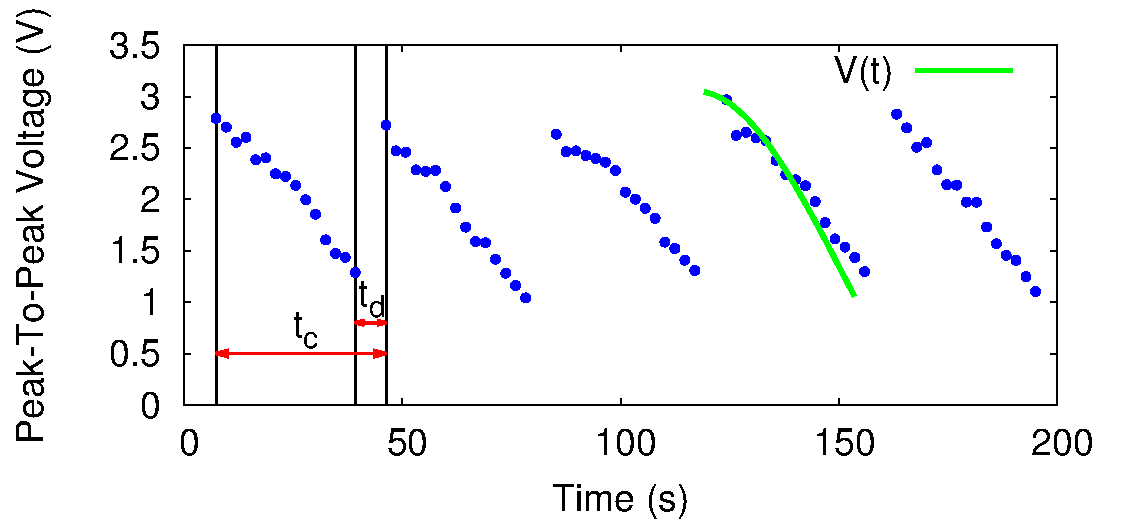
\includegraphics[width=\columnwidth]{figs/moving_recon.pdf}
\caption{Reconstruction voltage amplitude vs.\ time as the target moves along
one wall of the enclosure. A new sona signal is acquired every $t_{c}=39.8s$,
leading to a dead time of duration $t_{d}=7s$. The target is moving at a speed
of 0.5~$\frac{mm}{s}$ and the carrier frequency is 5~GHz.}
\label{fig:moving_recon}
\end{figure}
%%%%%%%%%%%%%%%%%%%%%%%%%%%%%%%%%%%%%%%%%%%%%%%%%%%%%%%%%%%%%%%%%%%%%%%%%%%%%%%%
